\begin{circuitikz}[scale=1.2, transform shape]

    \draw (2,-2) node [oscillator] (lo) {};
    \draw [color=blue] (lo.north) -- ++(0,0.5) -- ++(-1.5,0) -- ++(0,0.5);
    \draw [color=blue] (lo.south) -- ++(0,-0.5) -- ++(-1.5,0) -- ++(0,-0.5);
    %\draw [color=blue] (lo.south) to[short] ++ (0,-1) -- ++(-2.5,0) -- ++(0,-1);
    %\draw [color=blue] (2.5125, 1.5) -- ++ (0,-4) -- ++(-2.5,0) -- ++(0,-1);
    
    \draw (2,-2) node[right=0.1]{LO};
    
    \draw (0,0) node [mixer] (m1) {};
    \draw (m1.east) to [amp] (4,0)
    to [vR, rotate=0] (5.2,0) -- (6.5,0) -- (6.5, -1);
    %\draw (m1.east) to[short] ++(5,0) -- ++(0,-1)
    ;
    \draw (0,-4) node [mixer] (m2) {}
    (m2.east) to [short ]++(6,0) -- ++(0,1);

    %DAC outputs
    \draw (-0.45,0.25) to[short, -o] ++(-2,0) 
    (-0.45,-0.25) to[short, -o] ++(-2,0);
    \node () at (-1.5,0.5) {DAC I};
    \node () at (-1.5,-0.5) {DAC Q};
    %ADC inputs
    \draw (-0.45, -4+0.25) to[short, -o] ++(-2,0)
    (-0.45, -4-0.25) to[short, -o] ++(-2,0);
    \node () at (-1.5, -3.5) {ADC I};
    \node () at (-1.5, -4.5) {ADC Q};
    
     \draw [dash dot, rounded corners, fill=yellow, fill opacity=0.12] (5,-1) -- (8,-1) -- (8,-3) -- (5, -3) -- (5, -1)
    ;
    \node () at (7.5,-0.75) {Cryostat};
    
    \node[inner sep=0pt] (russell) at (6.5,-2) 
    {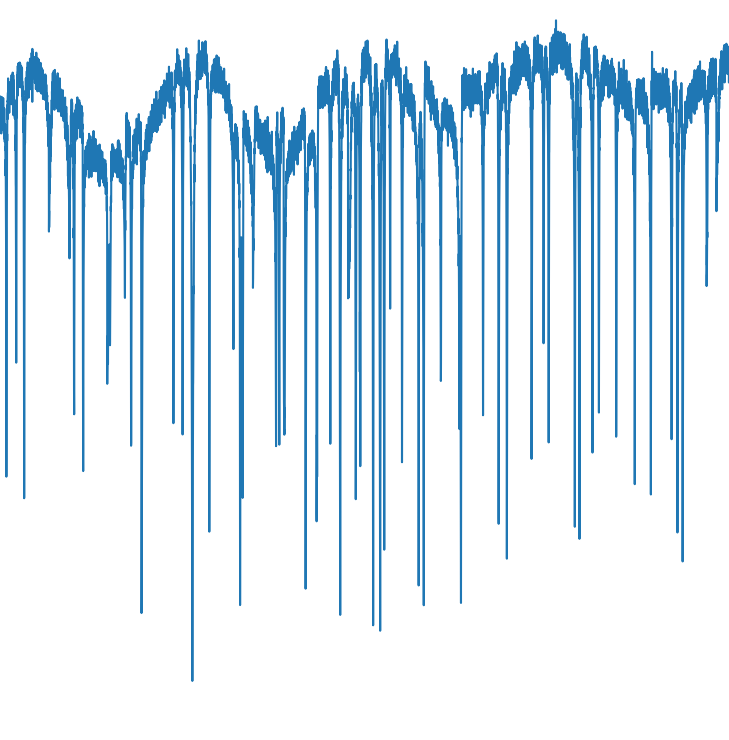
\includegraphics[width=.1\textwidth]{images/kid_example.png}};

    %\draw (5.5,-3) -- ++(0,-1);

    \draw [dash dot, rounded corners, fill=orange, fill opacity=0.12] (-2.5, 3.5) -- ++(0, -8) -- ++(-4,0) -- ++(0,8) -- ++(4,0)
    ; 
    \node () at (-4.5,2.75) {U-BOARD};

    \draw (1,0) -- ++(0,1.5) to [short, -o] (-2.45,1.5);
    \node () at (-1.5,1.75) {slow ADC};



\end{circuitikz}